% Created 2018-10-24 Wed 22:30
% Intended LaTeX compiler: pdflatex
\documentclass[11pt]{article}
\usepackage[utf8]{inputenc}
\usepackage[T1]{fontenc}
\usepackage{graphicx}
\usepackage{grffile}
\usepackage{longtable}
\usepackage{wrapfig}
\usepackage{rotating}
\usepackage[normalem]{ulem}
\usepackage{amsmath}
\usepackage{textcomp}
\usepackage{amssymb}
\usepackage{capt-of}
\usepackage{hyperref}
\author{UTL28}
\date{\today}
\title{}
\hypersetup{
 pdfauthor={UTL28},
 pdftitle={},
 pdfkeywords={},
 pdfsubject={},
 pdfcreator={Emacs 26.1 (Org mode 9.1.14)},
 pdflang={English}}
\begin{document}

\tableofcontents

\section{Graphics programming - home exam 1}
\label{sec:org4f102bb}
\subsection{Description of solution}
\label{sec:org0a16a86}
This report describes how I completed the first PG6200 home exam.

The end result is what I believe to be a functioning implementation of a shadow map algorithm.

\begin{center}
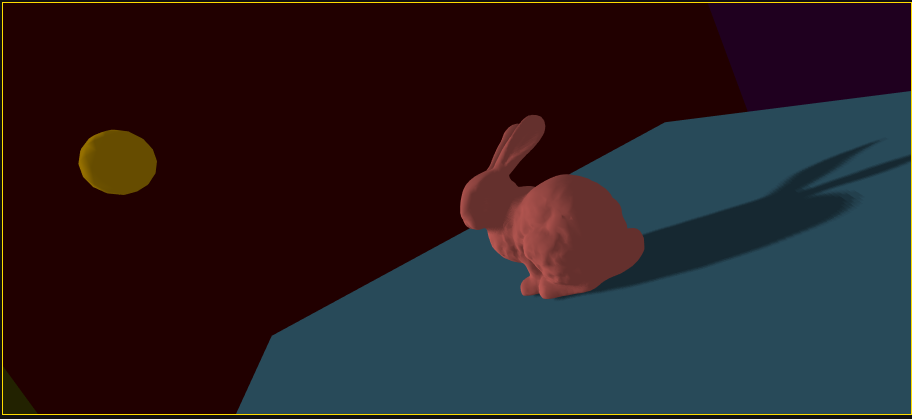
\includegraphics[width=.9\linewidth]{images/bunny_final.png}
\end{center}

Full disclosure:
The assignment states that you must have written all algorithms yourself, I cannot

\subsection{Technical challenges met during implementation}
\label{sec:orge846ce7}
The main challenge met during the implementation--which is likely to pop up other places in the report--was my lack of familiarity with WebGL as a whole. While I have made an effort to stay up to date and follow along with all the coursework, I recognize that I may not have succeeded completely, and as such, I must take at least part of the blame for this shortcoming.

The assignment states to use the data type \texttt{gl.UNSIGNED\_INT\_24\_8} for the texture. However, despite spending a lot of time looking for resources I was unable to find any that showed how to use this. The data type was mentioned several times, including in \href{https://developer.mozilla.org/en-US/docs/Web/API/WEBGL\_depth\_texture}{MDN's WebGL docs} and on \href{https://webgl2fundamentals.org/webgl/lessons/webgl-data-textures.html}{WebGLFundamentals}, but neither those nor any other resources I came across have any examples on how to use it.

Once I had managed to render to the texture and could confirm that it looked correct by rendering to the canvas instead of to the texture, the next thing was displaying the shadows correctly. In this I faced several challenges, of which the one that took me the longest to solve was how to make the shadows not be affected by the position and rotation of the camera. In the end I realized I had to multiply the lightModelViewMatrix by the camera's rotation matrix to make the shadows appear in the right spot.

Dimensions of the target texture. This is an area where I struggled to find any good information, but from what I could find, it seems the standard is to make it square. The larger you make it, the more information it can hold and the smoother your shadows will look due to the increased resolution that comes with the larger size. Naturally, this is a point where you trade performance for visual quality, but for keeping downtime to a minimum, I went with 1024x1024, which gives me fairly smooth shadows and still acceptable performance on a mid-range laptop.

There was also a fair amount of confusion relating to the orthographic projection matrix to be used for the light projection. In particular what values would be appropriate for the corners, and the near and far values. In the end it became a case of trial and error: finding something that would be able to capture the whole scene without getting too blurry because it's too far out. The ideal way to solve this would probably be to calculate how much has to be shown on a case by case basis and then rendering just the required amount, so that when the camera approaches an object and gets closer, the level of detail on the shadows would increase.


\subsection{Known bugs and probable causes}
\label{sec:org905fc24}
I had an issue with the shadow acne remover used in my fragment shader. At first it was much too coarse which caused the shadows to be severely reduced creating strange artefacts like the thick outline at the edges of the cube being lit when they were clearly in shadow. By making the acne remover much smaller I was able to greatly reduce the effect, but the issue still persists at a much smaller scale. It seems likely to be caused by a depth comparison issue, where the points along the edge are too close to what the point that the light hits and so is quite possibly caused by the depth texture resolution being too low. It could possibly also be caused by how the texture is set to wrap and/or the filters applied to it (\texttt{TEXTURE\_MIN\_FILTER\textasciitilde{}/\textasciitilde{}TEXTURE\_MAG\_FILTER}). A bit more time would have likely helped a fix for it.


\subsection{Testing methods utilized}
\label{sec:org022ed0d}
While I am very much an avid proponent of testing, there was no formal or rigorous testing used as part of this project. This is due in part to the fact that testing graphics is inherently more difficult as it can often be hard to test visuals, and due in part to the fact that WebGL is a very stateful system, where setting up test cases and assertions can be very difficult.

That said, one point where tests could have been very useful is in matrix multiplication and model transformations. If you knew what you would want to end up with, you could have set up a test case and written functions and refined them until they gave the desired output. However, this would require a very good understanding of exactly where you wanted to go and it sounds more like a tool for making sure your calculations and transformations are correct. That said, broken up into small enough functions, this could have been a good way to assert that transformations are correct and to detect potential regressions.

Furthermore, as my knowledge of WebGL is still very basic, the entire exercise has been in the realm some may describe 'exploratory programming', where you don't really know what you're going to end up with and how you're going to get there, but you do have an idea of the rough outlines of things. At this level, I would argue that proper testing is still more of an overhead than a boon. Once a proper architecture is established and a solid understanding of the system is in place, however, erecting a test suite would be very beneficial.

\subsection{Sources}
\label{sec:org062d6ea}
\url{https://webgl2fundamentals.org/webgl/lessons/webgl-render-to-texture.html}

\url{http://www.opengl-tutorial.org/intermediate-tutorials/tutorial-16-shadow-mapping/}

\url{http://www.chinedufn.com/webgl-shadow-mapping-tutorial/}
\end{document}